%%%%%%%%%%%%%%%%%%%%%%%%%%%%%%%%%%%%%%%%%
% Beamer Presentation
% LaTeX Template
% Version 1.0 (10/11/12)
%
% This template has been downloaded from:
% http://www.LaTeXTemplates.com
%
% License:
% CC BY-NC-SA 3.0 (http://creativecommons.org/licenses/by-nc-sa/3.0/)
%
%%%%%%%%%%%%%%%%%%%%%%%%%%%%%%%%%%%%%%%%%

%----------------------------------------------------------------------------------------
%	PACKAGES AND THEMES
%----------------------------------------------------------------------------------------

\documentclass{beamer}

\mode<presentation> {

% The Beamer class comes with a number of default slide themes
% which change the colors and layouts of slides. Below this is a list
% of all the themes, uncomment each in turn to see what they look like.

%\usetheme{default}
%\usetheme{AnnArbor}
%\usetheme{Antibes}
%\usetheme{Bergen}
%\usetheme{Berkeley}
%\usetheme{Berlin}
%\usetheme{Boadilla}
%\usetheme{CambridgeUS}
%\usetheme{Copenhagen}
%\usetheme{Darmstadt}
%\usetheme{Dresden}
%\usetheme{Frankfurt}
%\usetheme{Goettingen}
%\usetheme{Hannover}
%\usetheme{Ilmenau}
%\usetheme{JuanLesPins}
%\usetheme{Luebeck}
\usetheme{Madrid}
%\usetheme{Malmoe}
%\usetheme{Marburg}
%\usetheme{Montpellier}
%\usetheme{PaloAlto}
%\usetheme{Pittsburgh}
%\usetheme{Rochester}
%\usetheme{Singapore}
%\usetheme{Szeged}
%\usetheme{Warsaw}

% As well as themes, the Beamer class has a number of color themes
% for any slide theme. Uncomment each of these in turn to see how it
% changes the colors of your current slide theme.

%\usecolortheme{albatross}
%\usecolortheme{beaver}
%\usecolortheme{beetle}
%\usecolortheme{crane}
%\usecolortheme{dolphin}
%\usecolortheme{dove}
%\usecolortheme{fly}
%\usecolortheme{lily}
%\usecolortheme{orchid}
%\usecolortheme{rose}
%\usecolortheme{seagull}
%\usecolortheme{seahorse}
%\usecolortheme{whale}
%\usecolortheme{wolverine}

%\setbeamertemplate{footline} % To remove the footer line in all slides uncomment this line
%\setbeamertemplate{footline}[page number] % To replace the footer line in all slides with a simple slide count uncomment this line

%\setbeamertemplate{navigation symbols}{} % To remove the navigation symbols from the bottom of all slides uncomment this line
}

\usepackage{graphicx}
\usepackage{booktabs} 
\usepackage[T1]{fontenc}
\usepackage{lmodern}
\usepackage{textcomp}

%----------------------------------------------------------------------------------------
%	TITLE PAGE
%----------------------------------------------------------------------------------------

\title[Short title]{Pursue STEM: What Can You Do With Statistics?} % The short title appears at the bottom of every slide, the full title is only on the title page

\author{Nnenna Asidianya} % Your name
\institute[U of T] % Your institution as it will appear on the bottom of every slide, may be shorthand to save space
{
University of Toronto \\ % Your institution for the title page
\medskip
\textit{nnenna.asidianya@mail.utoronto.ca} % Your email address
}
\date{April 24th, 2021} % Date, can be changed to a custom date

\begin{document}

\begin{frame}
\titlepage % Print the title page as the first slide
\end{frame}

\begin{frame}
\frametitle{Outline} % Table of contents slide, comment this block out to remove it

\begin{enumerate}
	\item \textbf{Who} Am I?
	\item \textbf{What} do I do?
	\item  \textbf{When} did I decide to study statistics?
	\item \textbf{Where} was I in my life when I made this decision?
	\item \textbf{Why} did I make this change?
\end{enumerate}

\end{frame}


%------------------------------------------------


\begin{frame}
\frametitle{\textbf{Who} Am I?}
\begin{itemize}
	\item My name is Nnenna Asidianya. I am a second year statistics PhD student in the Department of Statistical Sciences (DOSS)
\end{itemize}
	\begin{center}
	
\includegraphics[width=0.4\linewidth]{me.jpg}
	\begin{figure}[H]
	\end{figure}
\end{center}


\end{frame}

%------------------------------------------------

\begin{frame}
\frametitle{ \textbf{What} do I do?}
\textbf{Recently years has seen an increase in the use of statistical methods by scientists in various fields. I have been actively involved in the following areas:}\\
\begin{itemize}
	\item Clinical Research 
	\item Statistical Education 
	\item Methodology 
\end{itemize}
\end{frame}

%------------------------------------------------

\begin{frame}
\frametitle{\textbf{What} do I do?}


	\begin{center}
	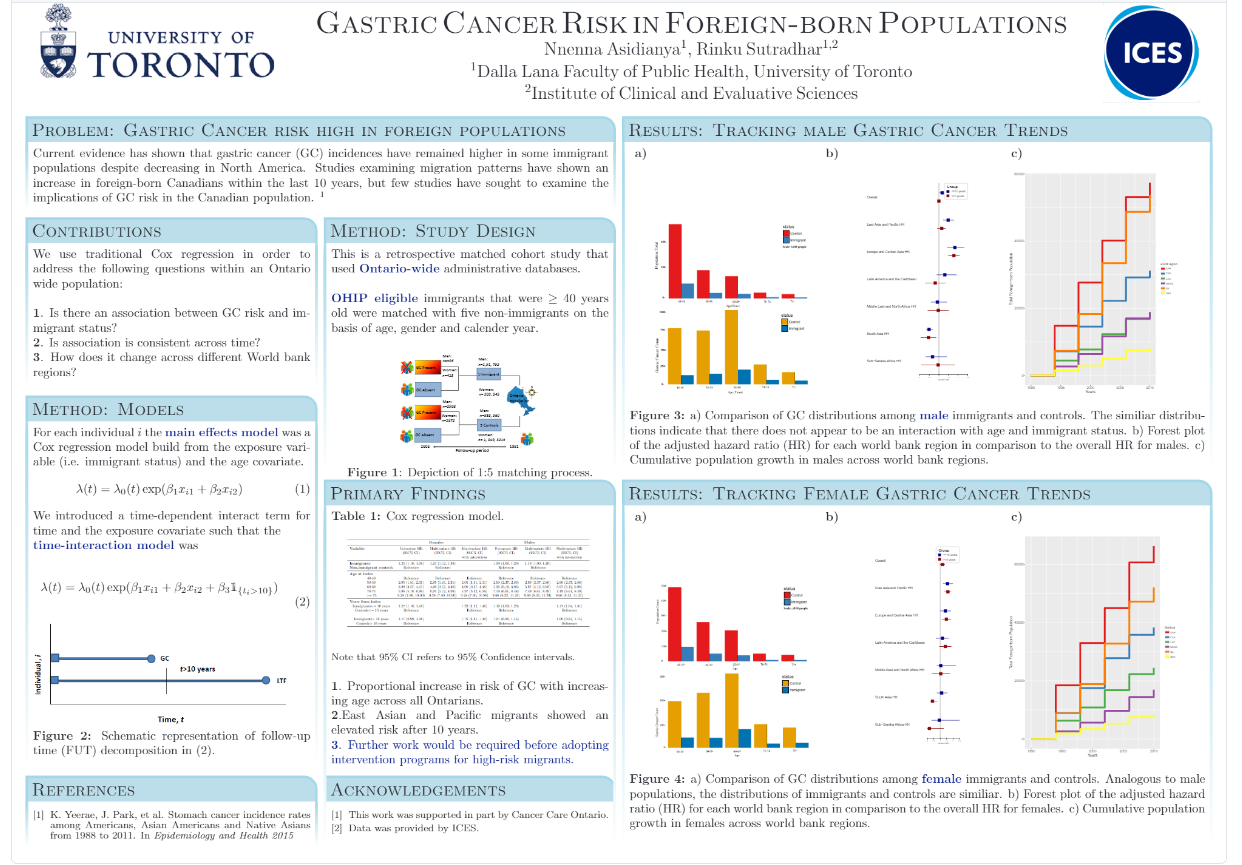
\includegraphics[width=0.95\linewidth]{gastric.png}
	\begin{figure}[H]
	\end{figure}
\end{center}

\end{frame}

%------------------------------------------------


\begin{frame}
\frametitle{\textbf{When} did I decide to study statistics?}
\begin{itemize}
\item First year courses: Biology I \& II, Chemistry I\& II, Physics I \& II, Calculus I\& II, \textit{\textcolor{red}{Electives: Statistics I}}
\item Second year courses: Organic chemistry I, Biochemistry I \& II, \textit{\textcolor{red}{ Electives: Linear Algebra I, Ordinary Differential Equations}}
\item Realization that I preferred my electives to my course courses.  
\item I began to take more mathematics courses in my second year of my undergraduate studies. 
\end{itemize}

\end{frame}

%------------------------------------------------
\begin{frame}
\frametitle{\textbf{Where} was I in my life when I made this decision?}
\begin{itemize}
	\item I am a second year student who began to take second year mathematics courses for self interest. 
	\item Ontario Shores Mental Health Research: Began working with SPSS statistical software in order to manage the data pertaining to satisfaction with inpatient care. 
	\item Realization that statistics was a driving force in clincal and medical research. 
	\item \textit{Officially took a major in statistics.}
\end{itemize}


\end{frame}
%------------------------------------------------

\begin{frame}
	\frametitle{\textbf{Why} did I make this change?}
	
		\begin{center}
		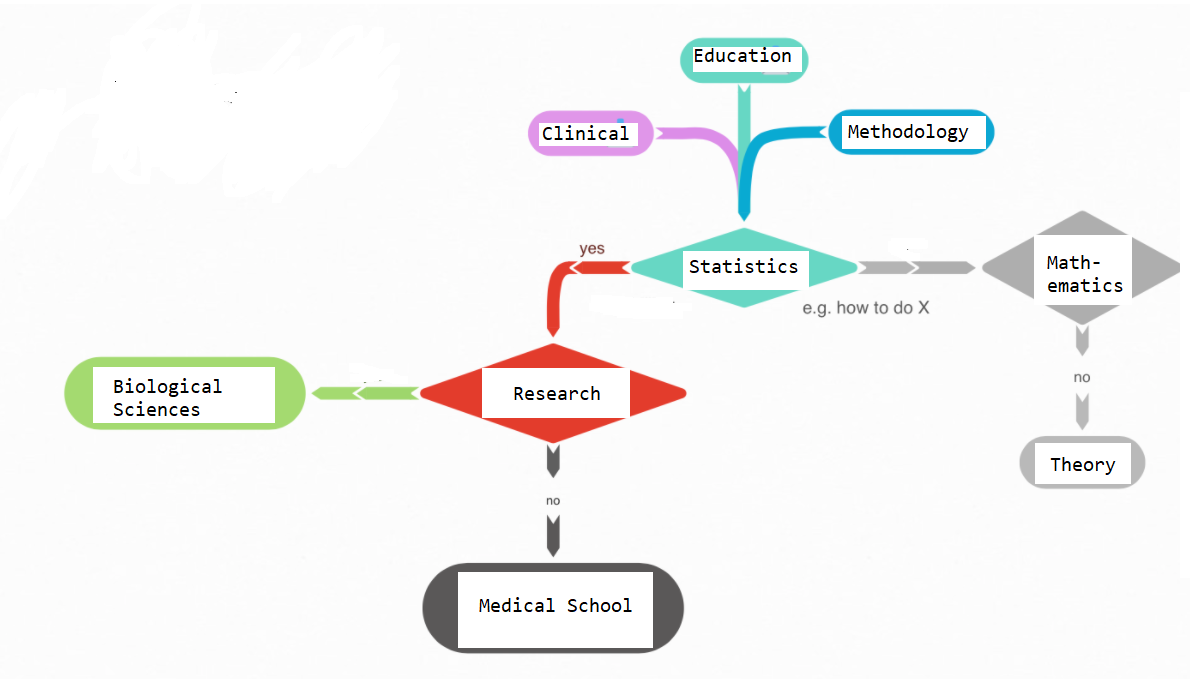
\includegraphics[width=1.0\linewidth]{map.png}
		\begin{figure}[H]
		\end{figure}
	\end{center}
	
\end{frame}

%------------------------------------------------

\end{document}